\section{سوال دوم}
تولید جواب مانند سوال سه تمرین دوم انجام شد. ابتدا یک رشته تصادفی با اعداد ۰ تا ۹ و دو عدد ۱- تولید شد. برای تولید جواب در همسایگی به صورت تصادفی دو عدد از رشته جواب مکانشان عوض می‌شد، این کار برای ۵۰ بار انجام می‌شد و در نهایت بهترین آنها انتخاب می‌شد و وارد لیست ممنوعه می‌شود. تابع هزینه به صورت کمترین زمان امداد رسانی مطرح شد. به این صورت، هر یک از هلیوکوپترها یک مسیری را طی می‌کردند که زمان کل امداد رسانی برابر با بیشترین مسافت طی شده است (فرض شده است که سرعت هلیکوپتر برابر با ۱ است.).

تولید لیست ممنوعه به این صورت است که اگر حرکتی انجام شد داخل لیست ممنوعه می‌رفت و اگر حرکتی داخل لیست ممنوعه بود انجام نمی‌شد. برای لیست ممنوعه یک طولی در نظر گرفته شده است که در ادامه به نحوه انتخاب اشاره شده است و هر زمان که لیست ممنوعه پر شد اولین عضو آن (قدیمی‌ترین عضو) از لیست خارج می‌شد و اخرین حرکت به اول لیست (جدیدترین عضو) به آن اضافه می‌شد. پارامترهای مساله شامل طول لیست ممنوعه و تعداد حرکات است که به صورت \lr{greedy}
با مقایسه نتایج انتخاب شده است. نتایج جدول بر اساس ده بار اجرا کد با شرایط نوشته شده است.
 	\lr{\begin{table}[H]
		\caption{Tabu list length study}
		\vspace{0.5cm}
		\centering
		\begin{tabular}{|c|c|c|c|}
			\hline
			Min & \lr{Standard deviation} & Mean & \lr{Tabu list length }  \\
			\hline 
			124.81 & 6.791 & 137.89 & 1000 \\
			118.16 & 8.622 &135.08 & 500\\
			126.01 & 8.23 &135.85 & 100\\
			\hline
		\end{tabular}
\end{table}}

 	\lr{\begin{table}[H]
		\caption{Number of iteration study}
		\vspace{0.5cm}
		\centering
		\begin{tabular}{|c|c|c|c|}
			\hline
			Min & \lr{Standard deviation} & Mean & \lr{Number of iteration}  \\
			\hline 
			124.81 & 6.791 & 137.89 & 10000 \\
			124.87 & 8.54 &141.86 & 5000\\
			137.93 & 14.80 &158.58 & 1000\\
			\hline
		\end{tabular}
\end{table}}

\begin{figure}[H]
	\caption{تابع هزینه بر حسب شماره تکرار} 
	\centering 
	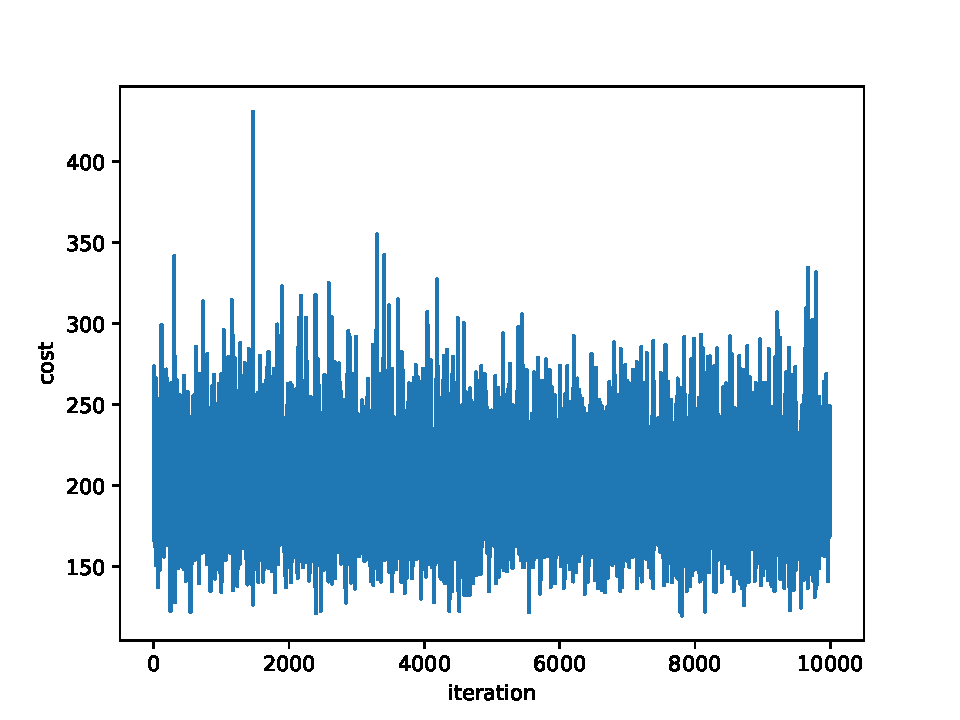
\includegraphics[width=12cm]{../Figure/Q2/tabu} 
\end{figure}
